%%% template.tex
%%%
%%% This LaTeX source document can be used as the basis for your technical
%%% paper or abstract.

%%% The parameter to the ``documentclass'' command is very important.
%%% - use ``review'' for content submitted for review.
%%% - use ``preprint'' for accepted content you are making available.
%%% - use ``tog'' for technical papers accepted to the TOG journal and
%%%   for presentation at the SIGGRAPH or SIGGRAPH Asia conference.
%%% - use ``conference'' for final content accepted to a sponsored event
%%%   (hint: If you don't know, you should use ``conference.'')

\documentclass[tog]{acmsiggraph}

\usepackage[ngerman]{babel}
\usepackage[utf8]{inputenc}
\usepackage{tikz}

%%% Make the ``BibTeX'' word pretty...

\def\BibTeX{{\rm B\kern-.05em{\sc i\kern-.025em b}\kern-.08em
    T\kern-.1667em\lower.7ex\hbox{E}\kern-.125emX}}

%%% Used by the ``review'' variation; the online ID will be printed on 
%%% every page of the content.

\TOGonlineid{45678}

%%% Used by the ``preprint'' variation.

\TOGvolume{0}
\TOGnumber{0}

\title{Ausarbeitung zum Thema der ganzzahligen lineare Programmierung (ILP)}

\author{Patric Vormstein\\Seminar Lineare und ganzzahlige lineare Programmierung, SoSe 2015\\Leitung: Prof. Dr. Ernst Althaus}
\pdfauthor{Stephen N. Spencer}

\keywords{radiosity, global illumination, constant time}

\begin{document}

%%% This is the ``teaser'' command, which puts an figure, centered, below 
%%% the title and author information, and above the body of the content.

 \teaser{
   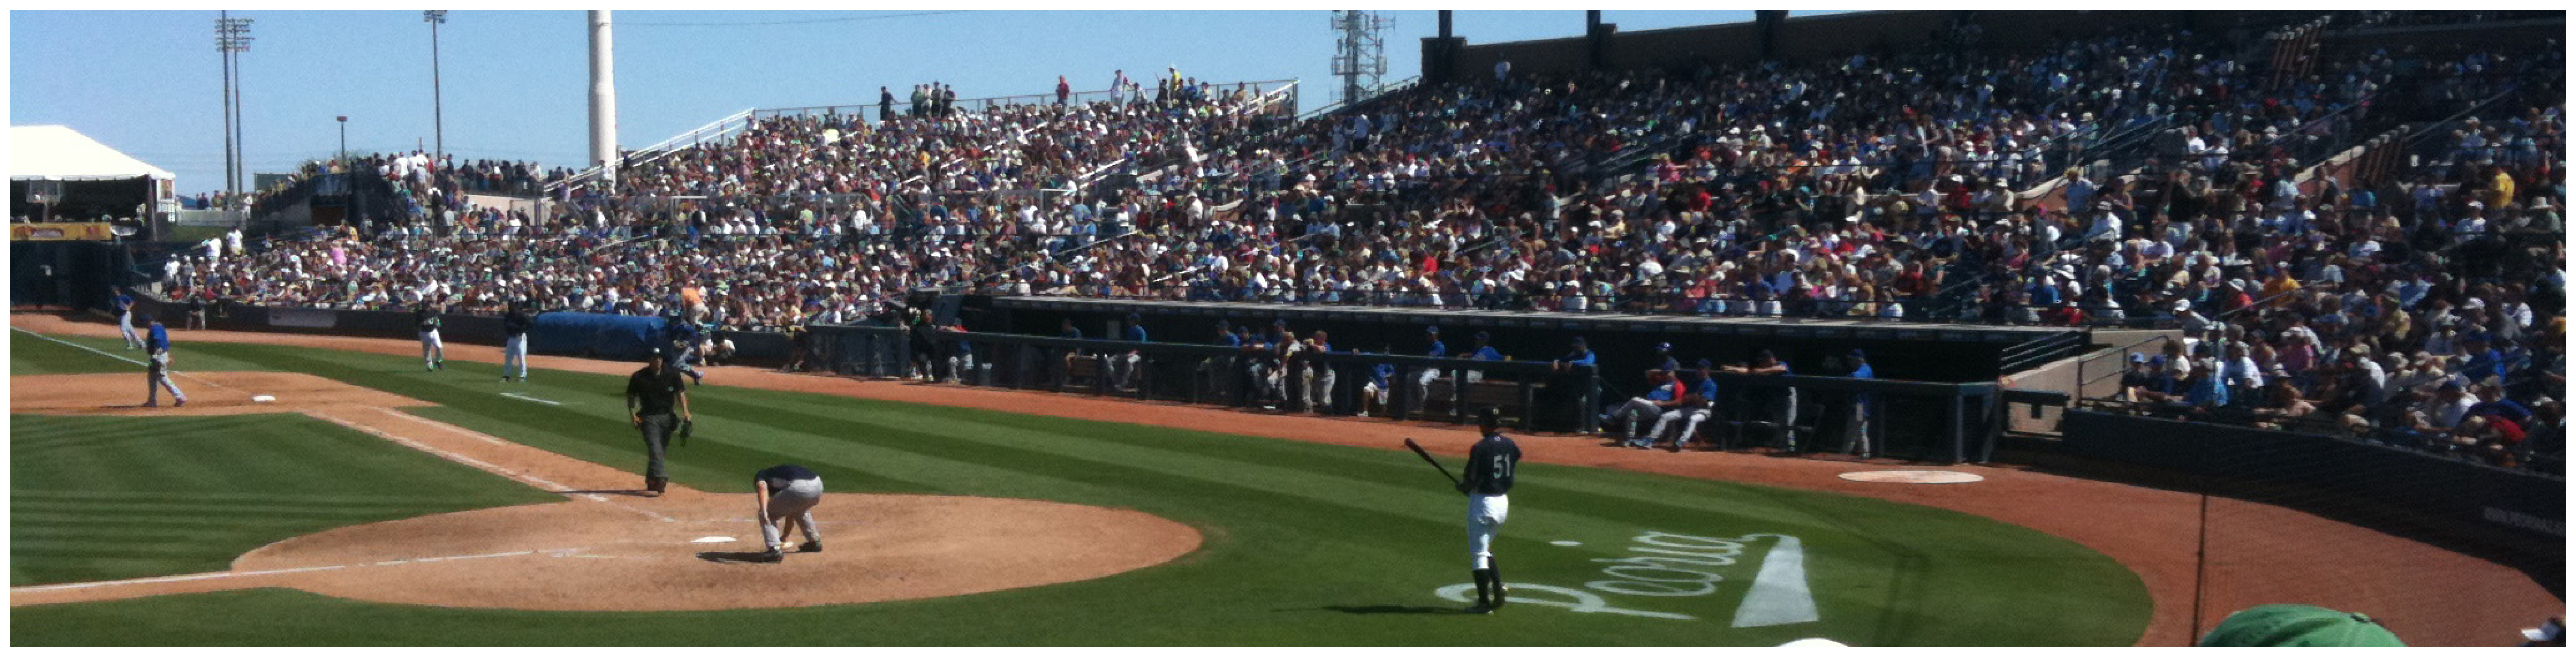
\includegraphics[height=1.5in]{images/sampleteaser}
   \caption{Spring Training 2009, Peoria, AZ.}
 }

\maketitle

\begin{abstract}

Diese Ausarbeitung setzt sich mit der ganzzahligen linearen Programmierung (oder ILP für \textit{integer linear programming}) auseinander und stellt drei exakte Algorithmen zum Lösen von ganzzahligen linearen Problemen vor.\\
Dabei handelt es sich um das Gomory-Schnittebenenverfahren, dem Branch-and-Bound-Algorithmus und ein Verfahren, dass die Vorteile beider Algorithmen nutzt, und zwar das Branch-and-Cut.\\
Ein besonderes Augenmerk soll hier auf die praktische Anwendung der Algorithmen gelegt werden.\\
Für diese Ausarbeitung werden nichtlineare Probleme, feasible bzw. zulässige Lösungen und der Simplex-Algorithmus (inkl. optimalem Tableau) als bekannt vorausgesetzt.\\
Desweiteren liegt dieser Ausarbeitung das Buch ... zugrunde.
\end{abstract}

%% Required for all content. 

%\copyrightspace

\section{Grundlagen}

Bevor auf die Algorithmen eingegangen wird müssen vorher noch die Grundlagen zu diesem Thema erläutert werden.\\
Als Anfangspunkt betrachten wir im Folgenden (\ref{Eq:LP}) eine bereits bekannte Form für ein generisches lineares Problem:

\large
\begin{align}
\label{Eq:LP}
minimize \;\; c'x & \nonumber \\
subject \;\; to \;\; Ax &= b \nonumber \\
x &\geq 0
\end{align}
\normalsize

Durch eine Modifikation der Lösungsvoraussetzung des Problems können wir das Problem in ein ganzzahliges Problem ändern. Wir beschränken die Lösungen auf Ganzzahligkeit. Dadurch erhalten wir folgende Form (\ref{Eq:ILP}) und somit eine ILP:

\large
\begin{align}
\label{Eq:ILP}
minimize \;\; c'x & \nonumber \\
subject \;\; to \;\; Ax &= b \nonumber \\
x &\geq 0 \nonumber \\
x \;\; &integer
\end{align}
\normalsize

Der Grund weshalb wir zuerst die nicht-ganzzahlige LP betrachtet haben liegt darin, dass sich jede ILP durch Wegnahme der Ganzzahligkeitsbeschränkung in eine sogenannte \textit{LP-Relaxierung} umwandeln lässt. Somit ist die LP aus der Gleichung \ref{Eq:LP} die LP-Relaxierung zur ILP aus Gleichung \ref{Eq:ILP}.

Die LP-Relaxierung dient dazu die Lösungssuche zu einer bestimmten ILP zu erleichtern, da es sich bei der Lösung von ILPs um ein NP-schweres Problem handelt. Daraus folgt, dass keine effizienten Algorithmen existieren.\\
Die Algorithmen denen man sich zur Lösung bedient lassen sich in drei Kategorien einteilen:

\begin{enumerate}
\item Exakte Algorithmen
\begin{itemize}
\item Berechnen eine optimale Lösung
\item Haben eine exponentielle Laufzeit
\end{itemize}
\item Approximierende Algorithmen
\begin{itemize}
\item Berechnen lediglich suboptimale Lösung
\item Haben dafür eine polynomielle Laufzeit
\end{itemize}
\item Heuristische Algorithmen
\begin{itemize}
\item Berechnen ohne Garantie eine suboptimale Lösung
\item Haben im besten Fall polynomielle Laufzeit, kann aber auch exponentiell sein
\item Meistens berechnen sie brauchbare Ergebnisse
\end{itemize}
\end{enumerate}

Die Algorithmen die wir in den folgenden Abschnitten beleuchten werden stammen aus der ersten Kategorie. Es handeln sich um exakte Algorithmen. 

\section{Schnittebenenverfahren}

Your content should be formatted on a US Letter (8.5 inches wide by 11
inches tall) page size. Please make sure you.re not working on an A4
page size. Page margins should be set at 0.75 inches on the right,
left, and top, and one inch at the bottom. Two columns should be used
throughout your content, except for the title, affiliations, and large
images or tables which span both columns.

To summarize, here are the basic page specifications: 
\begin{itemize}
\item page size: 8.5 inches wide by 11 inches wide (not A4)
\item top margin: 0.75 inches
\item right margin: 0.75 inches
\item left margin: 0.75 inches
\item bottom margin: 1 inch
\item number of columns: 2
\item column width: 3.3 inches
\item column height: 9.25 inches
\item column gutter: 0.33 inches
\end{itemize}

\section{Branch and Bound}

\begin{tikzpicture}[level/.style={sibling distance=60mm/#1}]
\node [circle,draw] (z){$F$}
	child { node [circle,draw] (a){$F_{1}$}
	}
	child { node [circle,draw] (b){$F_{2}$}
		child { node [circle,draw] (c){$F_{3}$}
		}
		child { node [circle,draw] (d){$F_{4}$}
		}
	}

;
\end{tikzpicture}

Please use a serif (Times, Times New Roman, etc.) typeface for the
body of your content. This serif typeface should be used for
everything except the title of your content and section headings,
which should be set in a sans-serif (Helvetica, etc.) typeface.

Your content should be prepared with 9-point text and 10-point line
spacing. This includes the references section. Do not reduce the
typeface size or the line spacing of any part of your content, in an
effort to fit more into a specific number of pages. 

All typefaces used in your content must be embedded in the PDF you
create. 

Paragraphs are prepared without any indentation on the first line, and
with a 10-point-tall space between paragraphs.

Please do not add page numbers to your content. They will be added
during production.

\section{Branch and Cut}

The title, author, and affiliation information should be centered
above the body of your content. The title should be set in a 14-point
bold sans-serif typeface with 18-point line spacing. The author and
affiliation information should be set in a 10-point serif typeface
with 12-point line spacing.

The title should be appropriately capitalized. ``All caps'' is not
appropriate. The following link provides assistance with appropriate
capitalization:

{\small\url{http://www.grammarbook.com/punctuation/capital.asp}}

Affiliations should include your educational institution or employer's
name, and a valid e-mail address.

\section{The Basics: Section Headings}

Section headings should be set in a 10-point bold sans-serif typeface
and numbered - ``1'', ``2'', and so on. Subsection headings should be
set in a 10-point bold sans-serif typeface and numbered - ``1.1'',
``1.2'', and so on. Subsubsection headings should be set in a 10-point
italic sans-serif typeface and numbered - ``1.2.1'', ``1.2.2'', and so
on. A 10-point-tall space should separate a section heading and the
next paragraph.

\section{Abstract, Keywords, and CR Categories}

Your content should begin with an abstract of about 150 words,
describing the work and its contribution to the field.

Authors of technical papers and technical briefs must also provide a
set of user-generated keywords and a selection of CR categories, from
the following link:

{\small\url{http://www.acm.org/about/class/1998/}}

Authors of other types of content may include CR categories and
keywords at their discretion.

\section{ACM Rights Management Text}

You are required to leave a blank space at the base of the left column
on the first page of your content for the ACM rights management
text. This blank space will be one column wide, and one inch tall for
all types of content except technical papers accepted to our annual
(SIGGRAPH and SIGGRAPH Asia) conferences. In this case, the space must
be 1.5 inches tall. (These technical papers are accepted as articles
in the ACM ``Transactions on Graphics'' journal, and the rights
management text is slightly different, and occupies more space.)

\section{Figures and Tables and Captions}

Figures and tables can span one or both columns. Captions for figures
should be centered underneath the figure. Captions for tables should
be centered above the table.

\begin{table}[ht]
  \centering
  \caption{A simple table.}
  \begin{tabular}{|r|l|}
    \hline
    7C0 & hexadecimal \\
    3700 & octal \\ \cline{2-2}
    11111000000 & binary \\
    \hline \hline
    1984 & decimal \\
    \hline
  \end{tabular}
\end{table}
  
Please use 9-point bold serif type for the caption title, and 9-point
serif type for the caption text (both on 10-point line spacing).

\section{Citations and References}

\subsection{Citations}

The SIGGRAPH citation format is the ``author year''
format~\cite{Pellacini:2005:LAH}. The year is separated from the
author by a single space~\cite{yee:2000:ssa}. Two authors are
separated by the word ``and''~\cite{parke:1996:CFA}. More than two
authors are represented by the primary author and ``et al.''~\cite{levoy:2000:TDM}.

Multiple citations at a single point in the content are separated by
semicolons~\cite{levoy:2000:TDM,sako:2001:SSB}.

When the last name of the cited author is part of the text, it may be
omitted from the citation: ``\ldots as shown in Fedkiw et
al.~\shortcite{fedkiw:2001:VSO}, the coefficient remains\ldots''

\subsection{References}

The reference list, or bibliography, must be unnumbered, alphabetized
by the primary author's last name, followed by the year of publication
and other identifying information (article title, journal title,
volume, number, etc.). Author names are arranged as ``last name,
initials.'' The page number, if any, is the last piece of information
in the reference.

The first line of each entry in the bibliography has no
indentation. The second successive lines has a 2em
indentation. 

Please use 9-point serif type, with 10-point line spacing, for each
entry in the bibliography, with a single blank line between each
entry. 

Journal, book, thesis, and conference proceedings titles are set in an
italic serif type. {\sc Author names should be typeset in a ``Small
Caps'' typeface.}

\section{Third-Party Material}

If you are using third-party material in your content - that is,
material which you or your co-authors did not create - you need to
clearly identify it as such in the material itself or in the 
content's caption, as shown in Figure~\ref{fig:ferrari}.

\begin{figure}[ht]
  \centering
  \includegraphics[width=3.0in]{images/ferrari_laferrari}
  \caption{Ferrari LaFerrari. Image courtesy Flickr user ``gfreeman23.''}
  \label{fig:ferrari}
\end{figure}

ACM's policy on third-party material can be found at the following link:

{\small\url{http://www.acm.org/publications/third-party-material}}

\section{``Artistic Images'' and Copyright Transfer}

ACM's rights management policy mandates that if copyright is
transferred to ACM, and authors wish to retain copyright of one or
more of their own images or figures in the content, they can identify
them as ``artistic images'' by including the author's copyright notice
in the image itself or in the caption.

(Please note that only technical papers and technical briefs have
copyright transfer as an option. All other forms of content have
permission and licensing options, but not copyright transfer.)

\section{Author-Prepared Versions of Final Content}

ACM's rights management policy provides for author-prepared versions
of final content to be made available on the author's personal or
employer's web site for distribution.

The author is responsible for creating the article-specific notice and
making it part of the PDF. The following is an example of such a
notice. Yours will have the year, publication, and article DOI
information specific to your final content.

\texttt{\small(c) 2009 ACM. This is the author's version of the work. It is posted here by permission of ACM for your personal use. Not for redistribution. The definitive version was published in ACM Transactions on Graphics 28(3), August 2009. http://doi.acm.org/10.1145/1576246.1531329.}

\section{Application-Specific Notes}

\subsection{\LaTeX}

The ``acmsiggraph'' \LaTeX{} class will faithfully implement the formatting specifications found in this document. Please look at the ``template.tex'' file that accompanies the \LaTeX\ and \BibTeX\ class files, noting these points:
\begin{itemize}
\item In order to leave the correct amount of space clear for the rights management text, you must do two things: 
\begin{enumerate}
\item Use the proper parameter to the \cs{documentclass} command at the top of your source file: use ``tog'' for technical papers accepted to our annual events and published as TOG articles, and use ``conference'' for all other types of content. The parameter determines the amount of space left clear for the rights management text.
\item Use the \cs{copyrightspace} command. It should be placed immediately before the first section of your paper.
\end{enumerate}
If you do not use any parameter to the \cs{documentclass} command, and use the \cs{copyrightspace} command, you'll end up with much more blank space than you want or need.

\item Many authors like to have a large image - called a ``teaser'' image - after the title, author, and affiliation and before the body of the paper. There is a command - \cs{teaser} - which can be used to place such an image. (As has been done in this example document.) Under certain circumstances, the space left clear for the rights management text will move to the base of the right column on the first page. This is acceptable.
\item Use the \cs{keywords} command to define your own keywords, and the \cs{keywordlist} command to prepare and print that block of text.
\item Use the \cs{CRcatlist} environment and the \cs{CRcat} command to define the CR categories appropriate for your paper.
\item There are also ``review'' and ``preprint'' variations of this document class, to be used for material submitted for review, and accepted content to be distributed as a ``preprint.'' These variations have special commands associated with them; see the ``template.tex'' file for more information.
\end{itemize}

\subsection{Microsoft Word}

The ``acmsiggraph.docx'' file will faithfully implement the formatting
specifications found in this document.

An appropriately-placed column break is one way to leave the right
amount of space for the rights management text.

\section{Proceedings Production}

Your final content will be checked and, if found acceptable for publication, will have the appropriate page header and footer information and ACM rights management text added to it. 

If your final content is not acceptable for publication - for example, unembedded typefaces, missing required elements, or modification of the format - you will be directed to correct these issues and submit a new version of your final content as soon as possible.

\section{Contact Information}

If you have questions or suggestions regarding this document, please
contact Stephen Spencer at ``spencer@cs.washington.edu''.

\section*{Acknowledgements}

To Robert, for all the bagels.

\bibliographystyle{acmsiggraph}
\nocite{*}
\bibliography{template}
\end{document}
